\documentclass{sig-alternate-per}


\usepackage{calc,xcolor}

\usepackage[utf8]{inputenc}
\usepackage[T1]{fontenc}
\usepackage{enumitem}

%\usepackage{amsmath,amsfonts,amsthm}
\newtheorem{theorem}{Theorem}
\newtheorem{coro}[theorem]{Corollary}
\usepackage{tikz}
\usepackage{hyperref}
\definecolor{darkblue}{rgb}{0 0 .6}
\hypersetup{colorlinks=true,linkcolor=darkblue,citecolor=darkblue,urlcolor=darkblue}
\hypersetup{pageanchor=false}
\usepackage{listings}

\newcommand{\vr}[1]{\mathbf{#1}}
\newcommand\MN{M^{(N)}}
\newcommand\XN{X^{(N)}}
\newcommand\LN{L^{(N)}}
\newcommand\DeltaN{\Delta^{(N)}}
\newcommand\bl{{\text{\boldmath$\ell$}}}
\newcommand\betaN{\beta^{(N)}}
\newcommand\PsiN{\Psi^{(N)}}
\newcommand\E{\mathcal{E}}
\newcommand\N{\mathbb{N}}
\newcommand\R{\mathbb{R}}
\newcommand\Z{\mathbb{Z}}
\newcommand\calL{\mathcal{L}}
\newcommand\floor[1]{\left\lfloor#1\right\rfloor}
\newcommand\var[1]{\mathrm{var}\left[#1\right]}
\newcommand\svar[1]{\mathrm{var}[#1]}
\newcommand\cov[1]{\mathrm{cov}\left[#1\right]}
\newcommand\scov[1]{\mathrm{cov}[#1]}
\newcommand\esp[1]{{\mathchoice{\besp{#1}}{\sesp{#1}}{\sesp{#1}}{\sesp{#1}}}}
\newcommand\besp[1]{\mathbb{E}\left[#1\right]}
\newcommand\sesp[1]{\mathbb{E}[#1]}
\newcommand\espN[1]{{\mathchoice{\bespN{#1}}{\sespN{#1}}{\sespN{#1}}{\sespN{#1}}}}
\newcommand\bespN[1]{\mathbf{E}^{(N)}\left[#1\right]}
\newcommand\sespN[1]{\mathbf{E}^{(N)}[#1]}
\newcommand\Proba[1]{{\mathchoice{\bProba{#1}}{\sProba{#1}}{\sProba{#1}}{\sProba{#1}}}} 
\newcommand\bProba[1]{\mathbf{P}\left[#1\right]}
\newcommand\sProba[1]{\mathbf{P}[#1]}
\newcommand\norm[1]{{\mathchoice{\bnorm{#1}}{\snorm{#1}}{\snorm{#1}}{\snorm{#1}}}}
\newcommand\bnorm[1]{\left\|#1\right\|}
\newcommand\snorm[1]{\|#1\|}
\newcommand{\n}[1]{m_{\mathit{#1}}}
\newcommand{\SET}[1]{\{#1\}}  

\newcommand\abs[1]{\left|#1\right|}
\newcommand\p[1]{\left(#1\right)}
\newcommand\dt{\frac{d}{dt}}
\newcommand\ds{\frac{d}{ds}}
\newcommand\Sym{\mathrm{Sym}}
\newcommand\red[1]{{\color{red!70!black!100}#1}}
\newcommand{\aN}{^{(N)}}
\newcommand\calU{{\mathcal{U}}}

\newcommand\J[1]{J_{(#1)}}

\graphicspath{{}{figs/}{../simu/}}

\begin{document}

\title{A Refined Mean Field Approximation for Synchronous Population
  Processes}%

\author{Nicolas Gast (Inria) \and Diego Latella (CNR-ISTI) \and Mieke
  Massink (CNR-ISTI)}

\maketitle

\begin{abstract}
  Mean field approximation is a popular method to study the behaviour
  of stochastic models composed of a large number of interacting
  objects. When the objects are asynchronous, the mean field
  approximation of a population model can be expressed as an ordinary
  differential equation. When the objects are synchronous the mean
  field approximation is a discrete time dynamical system.  In this
  paper, we focus on the latter. We show that, similarly to the
  asynchronous case, the mean field approximation of a synchronous
  population can be refined by a term in $1/N$. Our result holds for
  finite time-horizon and steady-state. We provide two examples that
  illustrate the approach and its limit.
\end{abstract}



\section{Introduction}

The idea behind mean field approximation is to replace the study of
the original stochastic system by the one of a, much simpler,
deterministic dynamical system.  Mean field approximation can be
applied to a variety of systems \cite{vvedenskaya1996queueing}; it can
be shown to be asymptotically optimal as the number of objects in the
system goes to infinity \cite{kurtz70,Le+07,benaim2008class} and is
often very accurate also for systems of moderate size, composed of
$N\approx100$ objects.

The mean field approximation of a given model is constructed by
considering the limit of the original stochastic model as the number
of objects $N$ goes to infinity. There can be two types of limits. The
first type arises when the dynamics of the objects are
asynchronous. In this case the mean field approximation is given by a
continuous time dynamical system (often a system of ordinary
differential equations) -- this is the most studied case \emph{e.g.}
\cite{kurtz70,benaim2008class,BHLM13}.  The second type arises when
the objects are synchronous. In this case the mean field approximation
is a discrete time dynamical system \cite{Le+07,gastgaujalDEDS}.  We
focus on the latter.

In this paper, we consider a variant of the (synchronous) population
models considered in \cite{Le+07,gastgaujalDEDS,latella2013fly}. Each
object evolves in a finite state-space and $\MN_i(t)$ denotes the
proportion of objects in a state $i$ at time $t$. The classical result
of \cite{Le+07} states if $\MN(0)=m$, then for any time $t$ the vector
$\MN(t)$ converges almost surely as $N$ grows to a deterministic
quantity $\mu(t)$ that satisfies the recurrence equation
\begin{align}
  \label{eq:mu}
  \mu(t+1)=\mu(t)\vr{K}(\mu(t))
\end{align}
with $\mu(0)=m$. Our contribution consists in computing the rate of
convergence : We show that there exists a time-dependent vector $V(t)$
such that
\begin{align}
  \label{eq:main_result}
  \esp{\MN(t)} = \mu(t) + \frac1N V(t) + o\p{\frac1{N}}. 
\end{align}
We show that $V(t)$ satisfies a linear dynamical system that involves
the first and second derivative of the function
$\Phi:m\mapsto m\vr{K}(m)$. Moreover, when $\Phi$ has a unique fixed
point $\mu(\infty)$ that is globally exponentially stable, then the
same result holds for the steady-state.

We call the quantity $\mu(t)+V(t)/N$ the \emph{refined} mean field
approximation. As opposed to the classical mean field approximation,
it depends on the system size $N$. We use two examples to show
that~:
\begin{itemize}[topsep=1pt,itemsep=0pt]
\item If the mean field approximation has a unique attractor that is
  exponentially stable, then our refined model is more accurate than
  the classical approximation uniformly in $t\in\R\cup\{\infty\}$.
\item When the mean field approximation does \emph{not} have an
  exponentially stable attractor, the improved accuracy only holds for
  a \emph{finite} time horizon.
\end{itemize}

Our results extend the recent results of \cite{gast2017refined}. The
authors of \cite{gast2017refined} study the steady-state of
asynchronous stochastic models (that therefore have a continuous-time
mean field approximation). There are two differences in our work :
First we focus on \emph{synchronous} objects; Second we obtain results
also for the \emph{transient} regime.  Note that the results of
\cite{gast2017refined} and the one of the current paper follow from a
series of recent results concerning the rate of convergence of
stochastic models to their mean field approximation
\cite{gast2017expected,kolokoltsov2011mean,ying2016rate}.

An extended version of the current paper has been accepted for
publication in \cite{GaLaMa17}. This paper and the simulations it
contained are fully reproducible~:
{\footnotesize\url{https://github.com/ngast/RefinedMeanField_SynchronousPopulation}}.

\section{Model and results}
\label{sec:model}



We consider a system of $N$ identical interacting objects; ($N$ is
called the {\em size} of the system).  Each object evolves in a finite
state space and the time is slotted. The vector $\MN(t)$ denotes the
occupancy measure at time $t$ : $\MN_j(t)$ is the {\em fraction} of
objects in state $j$ at $t$.

At each time step $t \in \N$, each object performs a local
transition. The transition probabilities of an object state depend on
the current local state of the object and may depend also on
$\MN(t)$. We denote by $K_{ij}(m)$ the probability for the object to
jump from state $i$ to state $j$ in the system given that $\MN(t)=m$.
We assume that, given the occupancy measure, the transitions made by
the objects are independent. Our model is identical to the one of
\cite{Le+07} up to the fact that the authors of \cite{Le+07} add a
continuous resource to the model and allow object transition matrix
$\vr{K}$ to depend also on the size $N$ of the system.  The results
presented in this paper could be easily extended to the more general
case.

The classical result (Theorem 4.1 of~\cite{Le+07}) shows that if
$M\aN(0)$ converges almost surely to the deterministic limit $\mu(0)$
as $N$ goes to infinity, then for any time $t>0$, $M\aN(t)$ converges
almost surely to $\mu(t)$ defined in Equation~\eqref{eq:mu}.


\subsection{First Main Result : Transient Behaviour}

Let $\Phi_t$ be the function defined recursively by $\Phi_1(m)=mK(m)$
and $\Phi_{t+1}(m)=\Phi_1(\Phi_t(m))$. We denote by $(D\Phi_1)(m)$ and
$(D^2\Phi_1)(m)$ the first and second derivative of the function
$\Phi_1$ evaluated in $m$.

\begin{theorem}\label{theo:main}
  Assume that the function $\Phi_1$ is twice differentiable and that
  $M\aN(0)$ converges weakly to $\mu(0)$. Let $A_t$ and $B_t$ be
  respectively the $n \times n$ matrix $A_t = (D \Phi_1)(\mu(t))$ and
  the $n \times n \times n$ tensor $B_t = (D^2 \Phi_1)(\mu(t))$.  Then
  \begin{align*}
    \lim_{N\rightarrow \infty} N\esp{M\aN(t)- \Phi_t(M\aN(0))} =
    V_t,
  \end{align*}
  where $V_t$ is a vector and $W_t$ is an $n \times n$ matrix defined
  by
  \begin{align}
    \begin{array}{rl}
      V_{t+1} & = A_tV_t + \frac{1}{2}B_t \cdot W_t\\
      W_{t+1} & = \Gamma(\mu(t)) + A_t W_t A_t^T,
    \end{array}
                \label{eq:VW}
  \end{align}
  with $V_0=0$, $W_0 = 0$ and $\Gamma({m})$ is the following
  $n \times n$ matrix:
  \begin{align*}
    \begin{array}{rl}
      \Gamma_{jj}({m}) & =  \sum_{i=1}^n m_i \vr{K}_{ij}({m})(1-\vr{K}_{ij}({m}))\\
      \Gamma_{jk}({m}) & = -\sum_{i=1}^n m_i \vr{K}_{ij}({m})\vr{K}_{ik}({m})
    \end{array}
  \end{align*}
\end{theorem}
The main idea is to consider a Taylor expansion of
$\esp{h(\Phi_1(m))}$ around $\Phi_1(m)$ for any function $h$ (see
\cite{GaLaMa17}).


\subsection{Second Main Result : Steady-State}
\label{ssec:steady}

Mean field approximation can also be used to characterise the
steady-state behaviour of a population model when the mean field
approximation has a unique attractor. Here, we show how to refine this
model when the mean field has an \emph{exponentially stable}
attractor, \emph{i.e.} a point $\mu(\infty)$ such that
\begin{itemize}[leftmargin=*]
\item $\mu(\infty)$ is an attractor: For any $m$ :
  $\lim_{t\to\infty}\Phi_t(m)=\mu(\infty)$.
\item $\mu(\infty)$ is exponentially stable : there exists $a,b>0$
  s.t. for all $m$ in a neighbourhood of $\mu(\infty)$ :
  $\norm{\Phi_t(m)-\mu(\infty)}\le a e^{-bt}\norm{m-\mu(\infty)}$.
\end{itemize}

\begin{theorem}\label{theo:steady}
  Assume that $\MN$ has a unique stationary distribution (for each
  $N$), that the function $\Phi_1$ is twice differentiable and that
  the flow has a unique exponentially stable attractor
  $\mu(\infty)$. Then there exists a $n\times1$ vector $V_{\infty}$ and
  a $n\times n$ matrix $W_{\infty}$ such that the constants $V_t$ and
  $W_t$ defined in Theorem~\ref{theo:main} satisfy:
  \begin{align*}
    \lim_{t\to\infty}V_t=V_{\infty} \qquad \mathrm{and}\qquad
    \lim_{t\to\infty}W_t=W_{\infty}
  \end{align*}
  Moreover
  \begin{itemize}[leftmargin=*]
  \item[(i)]$W_\infty$ is the unique solution of the discrete-time
    Lyapunov equation:
    \begin{align*}
      A_\infty WA_\infty^T - W + \Gamma(\mu(\infty)) = 0
    \end{align*}
    and $V_{\infty}=\frac12(I-A_\infty)^{-1}B_\infty W_\infty$ with
    $A_\infty=D\Phi_1(\mu(\infty))$, $B_\infty=D^2\Phi_1(\mu(\infty))$
    and $I$ is the identity matrix.
  \item[(ii)] We can exchange the limits :
    \begin{align*}
      &\lim_{N\to\infty}\lim_{t\to\infty}
        N\big(\mathbb{E}[\MN(t)]- \Phi_t(M\aN(0))\big)\\
      &=\lim_{t\to\infty}\lim_{N\rightarrow \infty}
        N\big(\mathbb{E}[\MN(t)]- \Phi_t({M}\aN(0))\big)
        = V_\infty. 
    \end{align*}
  \end{itemize}

\end{theorem}


\section{First example : SEIR}
\label{sect:RefSEIR}
In this section we provide a simple example that illustrates the
results for the refined mean field model of the simple computer
epidemic SEIR example presented in~\cite{BHLM13}.  Each object in the
model consists of four local states: Susceptible (S), Exposed (E),
Infected (I) (and active) and Recovered (R). 

Its discrete time evolution is given by the following probability
transition matrix $\vr{K}$ in which $\n{S}$, $\n{E}$, $\n{I}$ and
$\n{R}$ denote the fraction of objects in the system that are in local
state S, E, I and R:
\begin{align*}
  \vr{K}(m)
  = \left(
  \begin{array}{cccc}
    1 - (\alpha_e + \alpha_i\n{I}) & \alpha_e + \alpha_i \n{I} & 0 & 0  \\
    0 & 1- \alpha_a & \alpha_a & 0 \\
    0 & 0 & 1 - \alpha_r & \alpha_r \\
    \alpha_l & 0 & 0 & 1 - \alpha_l 
  \end{array}
  \right)
\end{align*}
In other words, a susceptible becomes exposed with probability
$(\alpha_e+\alpha_i m_I)$ -- \emph{i.e.}, $\alpha_e$ denotes the
external and $\alpha_i$ the internal infection probability --; An
exposed node activates his infection with probability $\alpha_a$; An
infected recovers with probability $\alpha_r$; and $\alpha_l$ is the
probability to loose the protection against infection.


To give an idea of how the refined mean field approximation improves
the accuracy compared to the classical mean field approximation, we
plot in Figure~\ref{fig:diff} the difference between the two
approximations with respect to the simulation~: On the left panel, we
plot $\esp{\MN(t)}-\mu(t)$; On the right panel we plot
$\esp{\MN(t)}-(\mu(t)+V(t)/N)$ (in both cases for $N=10$). The
expectation was computed by using an average of 50,000 runs of a
stochastic simulation of the model.  The values of the parameters
are~: $\alpha_e=0.01, \alpha_i=0.08,\alpha_r=0.02,\alpha_l=0.01$ and
$\alpha_a=0.04$. and the initial state was $M_S(0)=1$ and
$M_E(0)=M_I(0)=M_R(0)=0$.
\begin{figure}[ht]
  \begin{center}
    \begin{tabular}{cc}
      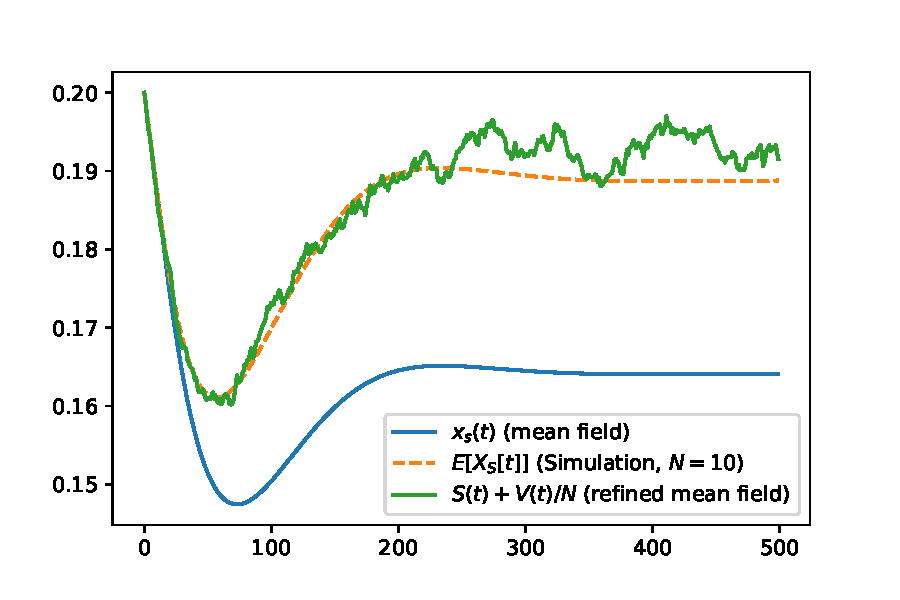
\includegraphics[width=0.45\linewidth]{SEIR_errorMF_N10}
      &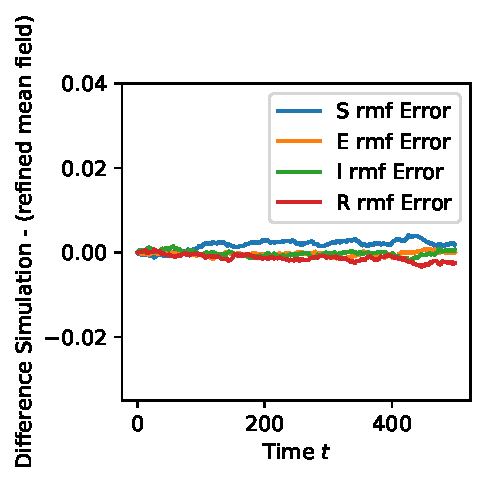
\includegraphics[width=0.45\linewidth]{SEIR_errorRMF_N10}\\
      Error of mean field approx.
      &
        Error of the refined approx.
    \end{tabular}\vspace{-.2cm}
  \end{center}
  \caption{\label{fig:diff} SEIR model: Quantification of the error of
    the mean field or refined mean field approximation ($N=10$).}
\end{figure}

We observe that the refined mean field approximation (right panel) is
an order of magnitude closer to the value obtained by simulation. This
figure illustrates that Theorem~\ref{theo:main} is not just valid
asymptotically, but actually it refines the classical mean field
approximation for relatively small values of $N$. In this case, the
system has a unique attractor and the refined approximation can be
used for estimating the steady-state expected values (see
Table~\ref{tbl:steadySEIR}).

 \begin{table}[ht]
\begin{center}
\begin{tabular}{@{}|@{~}c@{~}|c|c|c|c|}\hline
State                                & $S$ & $E$ & $I$ & $R$ \\\hline
Simulation ($N=10$)            & 0.191 & 0.115 & 0.231 &0.462 \\ \hline
Refined mean field ($N=10$) & 0.189& 0.116 & 0.232& 0.464\\ \hline
Mean field ($N=10$)               & 0.164 & 0.119 & 0.239 & 0.478\\ \hline
\end{tabular}
\end{center}
\caption{\label{tbl:steadySEIR} SEIR model: Comparison of the accuracy
  of the mean field and refined mean field approximation for the
  steady-state proportion of objects in states $S$, $E$, $I$ or $R$. }
\end{table}
   

\section{Accuracy versus Time}

In the previous example, the mean field limit has an exponentially
stable attractor, which implies that the accuracy of the mean field
approximation is uniform in time (Theorem~\ref{theo:steady}(ii)).
Here, we show that this is no longer the case if the model does not
have an exponentially stable attractor.

We consider a system with $N$ objects in which each object is in state
$0$ or $1$. An object in state $1$ goes to state $0$ with probability
$1$ and an object in state $0$ goes to $1$ with probability
$\alpha m_0$, where $\alpha\in(0,1)$ is a parameter. The transition
matrix $K$ is therefore
\begin{align*}
  K(m) = \left[
  \begin{array}{cc}
    1-\alpha m_0&\alpha m_0\\
    1 & 0
  \end{array}
\right]
\end{align*}
The function $m\mapsto mK(m)$ has a unique fixed point whose first
component is $\mu_0(\infty)=(\sqrt{1+4\alpha}-1)/(2\alpha)$. This
fixed point is exponentially stable if and only if $\alpha < 0.75$.

In Figure~\ref{fig:stable} and Figure~\ref{fig:unstable}, we plot the
mean field $\mu(t)$ and refined mean field approximation
$\mu(t)+V(t)/N$ as well an exact value of $\esp{M(t)}$ for $N=10$ and
$N=30$. The initial value is $m(0)=0.7$. The exact value of
$\esp{M(t)}$ was computed by a numerical method that uses the fact
that the system with $N$ objects can be described by a Markov chain
with $N+1$ states.

These figures show that the refined approximation always improves the
accuracy compared to the classical mean field approximation for small
values of $t$, both for $\alpha=0.6$ and $\alpha=0.75$. The situation
for large values of $t$ is quite different. On the one hand, when the
fixed point is exponentially stable ($\alpha=0.6$,
Figure~\ref{fig:stable}), the refined approximation is very accurate
for all values of $t$. On the other hand, when the fixed point is not
exponentially stable ($\alpha=0.75$, Figure~\ref{fig:unstable}), the
refined approximation seems to be unstable and is not a good
approximation of $\esp{M(t)}$ for values of $t$ that are too large
compared to $N$ ($t>7$ for $N=10$ or $t>12$ for $N=30$).

\begin{figure}[ht]
  \centering
  \begin{tabular}{@{}c@{}c@{}}
    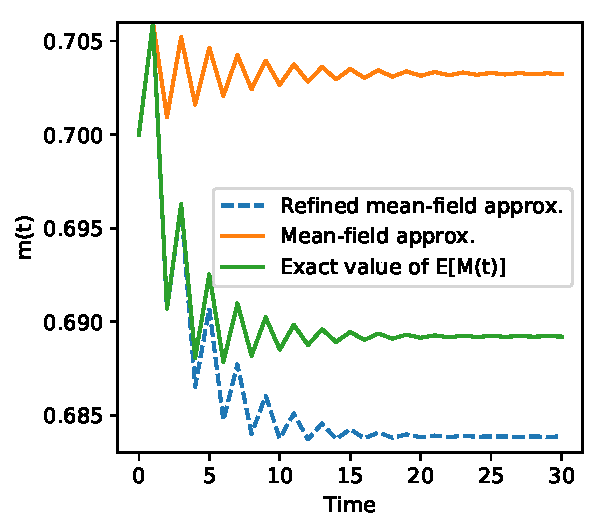
\includegraphics[width=.5\linewidth]{unstable1D_a60_N10}
    &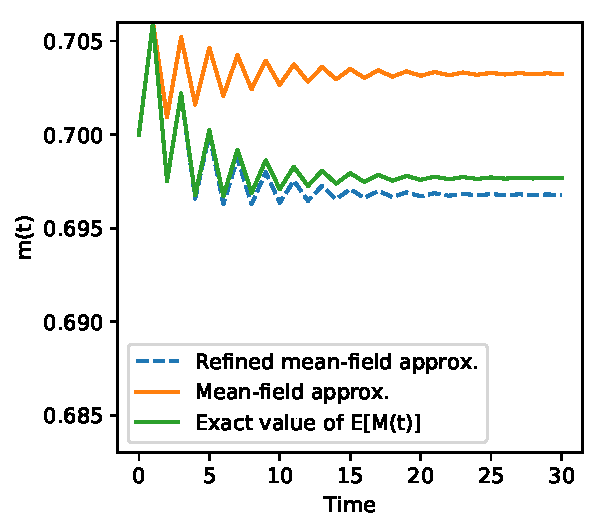
\includegraphics[width=.5\linewidth]{unstable1D_a60_N30}\\
    (a) $N=10$ & (b) $N=30$
  \end{tabular}
  \caption{Exponentially stable case ($\alpha=0.6$).}
  \label{fig:stable}
\end{figure}

\begin{figure}[ht]
  \centering
  \begin{tabular}{@{}c@{}c@{}}
    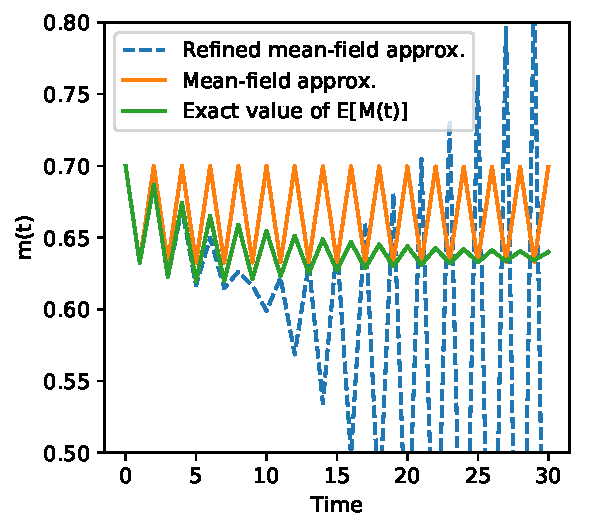
\includegraphics[width=.5\linewidth]{unstable1D_a75_N10}
    &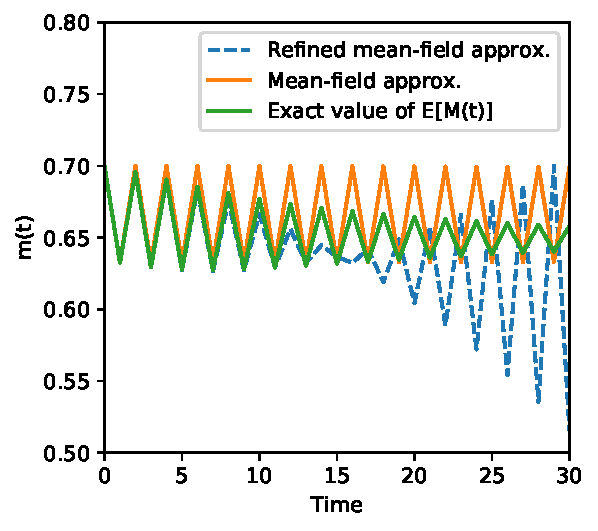
\includegraphics[width=.5\linewidth]{unstable1D_a75_N30}\\[-5pt]
    (a) $N=10$ & (b) $N=30$\vspace{-.3cm}
  \end{tabular}
  \caption{Non-exponentially stable case ($\alpha=0.75$). }
  \label{fig:unstable}
\end{figure}

\section{Conclusion and Extensions}

In this paper, we have shown that it is possible to adapt the refined
mean field approximation proposed in \cite{gast2017refined} to the
case of synchronous population processes, both for transient and
steady-state state. This approximation is more accurate than the
classical mean field approximation in many cases. Yet, when the mean
field approximation does not have an exponentially stable attractor,
this new approximation must be handle with care. We are currently
working on extending this methodology to study the transient regime of
asynchronous population processes, in which case
Equation~\eqref{eq:VW} can be replaced by an ordinary differential
equation.

\small 
% \bibliographystyle{ACM-Reference-Format}
\bibliographystyle{plain}
\bibliography{RefMeanField.bib}

\end{document}

